\documentclass[11pt]{article}

% ============================================================
% PACKAGES  (kept to what is actually installed on this machine —
%  no tcolorbox / mdframed / enumitem / titlesec; all boxes below
%  are hand-rolled with xcolor rules so they break safely across pages)
% ============================================================
\usepackage[T1]{fontenc}
\usepackage{amsmath,amssymb,amsthm,mathtools}
\usepackage{geometry}
\geometry{letterpaper,margin=1in}
\usepackage{xcolor}
\usepackage{graphicx}
\usepackage{tikz}
\usepackage{booktabs}
\usepackage{longtable}
\usepackage{array}
\usepackage{parskip}
\usepackage{fancyhdr}
\usepackage[colorlinks=true,linkcolor=linkblue,citecolor=linkblue,urlcolor=linkblue,
            bookmarksnumbered=true,pdfborder={0 0 0}]{hyperref}
\usepackage{bookmark}

% ============================================================
% COLORS
% ============================================================
\definecolor{linkblue}{RGB}{20,60,130}
\definecolor{defcol}{RGB}{20,80,160}
\definecolor{defbg}{RGB}{235,242,250}
\definecolor{thmcol}{RGB}{20,120,90}
\definecolor{thmbg}{RGB}{232,246,240}
\definecolor{flagcol}{RGB}{170,30,30}
\definecolor{flagbg}{RGB}{253,235,235}
\definecolor{exmcol}{RGB}{110,60,150}
\definecolor{exmbg}{RGB}{243,236,250}
\definecolor{notecol}{RGB}{180,110,10}
\definecolor{notebg}{RGB}{252,244,225}
\definecolor{examcol}{RGB}{40,40,40}

% ============================================================
% MATH SHORTCUTS
% ============================================================
\newcommand{\E}[1]{\mathrm{E}\left[#1\right]}
\newcommand{\Var}[1]{\mathrm{Var}\left[#1\right]}
\newcommand{\Cov}[1]{\mathrm{Cov}\left[#1\right]}
\newcommand{\ddx}{\,d}
\renewcommand{\P}[1]{P\left[#1\right]}

% ============================================================
% HAND-ROLLED, PAGE-BREAK-SAFE BOXES (rule above/below + colored bold heading)
% ============================================================
\newcommand{\topline}[1]{\par\vspace{5pt}\noindent{\color{#1}\rule{\linewidth}{1.1pt}}\par\vspace{3pt}}
\newcommand{\botline}[1]{\par\vspace{2pt}\noindent{\color{#1}\rule{\linewidth}{1.1pt}}\par\vspace{8pt}}

\newenvironment{defbox}[2]{%
  \topline{defcol}\noindent\textbf{\color{defcol}Definition #1 --- #2}\par\smallskip\noindent\ignorespaces
}{\botline{defcol}}

\newenvironment{thmbox}[2]{%
  \topline{thmcol}\noindent\textbf{\color{thmcol}Theorem #1 --- #2}\par\smallskip\noindent\ignorespaces
}{\botline{thmcol}}

\newenvironment{flagbox}[2]{%
  \topline{flagcol}\vspace{-9pt}\topline{flagcol}%
  \noindent\textbf{\color{flagcol}$\bigstar$ Theorem #1 --- #2 $\bigstar$ \; [PROFESSOR-FLAGGED --- MEMORIZE]}\par\smallskip\noindent\ignorespaces
}{\botline{flagcol}\vspace{-9pt}\botline{flagcol}}

\newenvironment{exbox}[2]{%
  \topline{exmcol}\noindent\textbf{\color{exmcol}Example #1 --- #2}\par\smallskip\noindent\ignorespaces
}{\botline{exmcol}}

\newenvironment{notebox}[1]{%
  \topline{notecol}\noindent\textbf{\color{notecol}#1}\par\smallskip\noindent\ignorespaces
}{\botline{notecol}}

\newenvironment{examprob}[2]{%
  \topline{examcol}\noindent\textbf{\color{examcol}#1 --- #2}\par\smallskip\noindent\ignorespaces
}{\botline{examcol}}

% quick inline "how to use" formula chip
\newcommand{\keyresult}[1]{%
  \par\noindent\fcolorbox{thmcol}{thmbg}{\parbox{\dimexpr\linewidth-2\fboxsep-2\fboxrule}{\textbf{Key takeaway:} #1}}\par\smallskip}

% ============================================================
% HEADER / FOOTER
% ============================================================
\pagestyle{fancy}
\fancyhf{}
\fancyhead[L]{\footnotesize\itshape Final Exam Master Guide}
\fancyhead[R]{\footnotesize\itshape \leftmark}
\setlength{\headheight}{14pt}
\fancyfoot[C]{\thepage}
\renewcommand{\headrulewidth}{0.4pt}

\setcounter{tocdepth}{3}
\setcounter{secnumdepth}{3}
\tolerance=1400
\emergencystretch=3em
\hbadness=3000
\hfuzz=2pt

\title{\Huge\textbf{Probability \& Stochastic Processes}\\[6pt]
\Large Final Exam Master Reference Guide\\[4pt]
\large Chapters 4, 5, 6 \& 13}
\author{}
\date{Compiled for Final Exam Review}

% ============================================================
\begin{document}
\pagenumbering{roman}
\begin{titlepage}
\centering
\vspace*{2cm}
{\Huge\bfseries Probability \& Stochastic Processes}\\[10pt]
{\LARGE Final Exam Master Reference Guide}\\[6pt]
{\Large\itshape Every Theorem You Need, Fully Worked}\\[40pt]

{\large\bfseries Scope of This Guide}\\[8pt]
\begin{minipage}{0.82\linewidth}
\centering
Chapter 4: \S4.2--4.3 (CDF/PDF), \S4.6 (Gaussian RVs), \S4.7 (Delta Functions \& Mixed RVs)\\[4pt]
Chapter 5: \S5.7 (E[g(X,Y)]), \S5.8 (Covariance/Correlation), \S5.9 (Bivariate Gaussian)\\[4pt]
Chapter 6: \S6.2 (Functions Yielding Continuous RVs), \S6.3 (Functions Yielding Discrete/Mixed RVs)\\[4pt]
Chapter 13: \S13.7--13.11 (Stochastic Processes: Stationarity, WSS, Ergodicity, Cross-Correlation, Gaussian Processes)\\[10pt]
\end{minipage}

\vspace{25pt}
\fcolorbox{flagcol}{flagbg}{%
\begin{minipage}{0.78\linewidth}
\centering\vspace{4pt}
\textbf{\color{flagcol}Professor's Exact Guidance (verbatim)}\\[6pt]
\itshape ``The final is made up. I will be giving you the exact sheet from the first exam,
so anything from chapter 5, 6 and 13 --- that's what you should concentrate your notes on.
There will be a section of the test where you will have a choice based on the material and
chapters 4, 5 and 6. There will also be two questions on chapter 13.''
\vspace{4pt}
\end{minipage}}

\vfill
{\large Textbook: Yates \& Goodman, \textit{Probability and Stochastic Processes}, 3rd edition}\\[4pt]
{\normalsize Cross-checked against Exam 1 and Exam 2 solution keys}
\vspace{1cm}
\end{titlepage}

\clearpage
\tableofcontents
\clearpage
\pagenumbering{arabic}

% ================================================================
\section*{How This Guide Is Organized}
\addcontentsline{toc}{section}{How This Guide Is Organized}

Every \textbf{Definition} appears in a \textcolor{defcol}{\textbf{blue}} rule-box, every
\textbf{Theorem} in a \textcolor{thmcol}{\textbf{green}} rule-box, every worked
\textbf{Example} in a \textcolor{exmcol}{\textbf{purple}} rule-box, and every explicit
professor-emphasized remark in an \textcolor{notecol}{\textbf{orange}} rule-box. Theorems the
professor personally flagged on the review sheet (Theorem 13.10, 13.11, 13.12, and Example
13.22) get a special double-rule \textcolor{flagcol}{\textbf{red}} box with a $\bigstar$ ---
\textbf{these are the highest-priority items to memorize}. Every Theorem/Definition number
matches the exact number used in Yates \& Goodman, 3rd edition, so you can cross-reference
directly with your textbook or the professor's exam-1 sheet. Part~\ref{part:exams} reproduces
\emph{every single problem} from Exam 1 and Exam 2 with complete, checked, step-by-step
solutions, tagged by topic. Part~\ref{part:cheatsheet} is a dense one-page-style formula
cheat-sheet for last-minute review.

\clearpage
% ================================================================
\part{Chapter 4 --- Continuous Random Variables}
% ================================================================
\section{The CDF and PDF (\S4.2--4.3): Foundations}

\subsection{The Cumulative Distribution Function}

\begin{defbox}{4.1}{Cumulative Distribution Function (CDF)}
The CDF of random variable $X$ is
\[ F_X(x) = \P{X \le x}. \]
This is a probability model for \emph{any} random variable --- discrete, continuous, or mixed.
$F_X(x)$ is a continuous function \emph{if and only if} $X$ is a continuous random variable.
\end{defbox}

\begin{thmbox}{4.1}{Basic CDF Properties}
For any random variable $X$:
\begin{align*}
\text{(a)}\quad & F_X(-\infty) = 0 \\
\text{(b)}\quad & F_X(\infty) = 1 \\
\text{(c)}\quad & \P{x_1 < X \le x_2} = F_X(x_2) - F_X(x_1).
\end{align*}
$F_X$ is nondecreasing; for \emph{discrete} $X$ it is a jump-staircase (jump size $=P_X(x)$
at each $x\in S_X$); for \emph{continuous} $X$ it is continuous everywhere (this continuity
\emph{is} the definition of ``continuous r.v.'').
\end{thmbox}

\begin{defbox}{4.2}{Continuous Random Variable}
$X$ is continuous if and only if its CDF $F_X(x)$ is a continuous function of $x$.
\end{defbox}

\subsection{The Probability Density Function}

\begin{defbox}{4.3}{Probability Density Function (PDF)}
For a continuous random variable $X$,
\[ f_X(x) = \frac{dF_X(x)}{dx}. \]
The PDF is the single most useful complete probability model of a continuous r.v.: its graph
shows directly which values are likely.
\end{defbox}

\begin{thmbox}{4.2}{Basic PDF Properties}
\begin{align*}
\text{(a)}\quad & f_X(x)\ge 0 \text{ for all } x \\
\text{(b)}\quad & F_X(x) = \int_{-\infty}^{x} f_X(u)\,du \\
\text{(c)}\quad & \int_{-\infty}^{\infty} f_X(x)\,dx = 1.
\end{align*}
\end{thmbox}

\begin{thmbox}{4.3}{Interval Probability from the PDF}
\[ \P{x_1 < X \le x_2} = \int_{x_1}^{x_2} f_X(x)\,dx. \]
\end{thmbox}

\begin{notebox}{Critical Exam Reminder}
The PDF value $f_X(x)$ is \emph{not} a probability --- it can exceed 1. Only \emph{areas}
under $f_X$ are probabilities. Because $\P{X=x}=0$ for continuous $X$, all four events
$\{x_1{<}X{<}x_2\}$, $\{x_1{\le}X{<}x_2\}$, $\{x_1{<}X{\le}x_2\}$, $\{x_1{\le}X{\le}x_2\}$ have
the \emph{same} probability. This is \textbf{false} for discrete/mixed random variables ---
watch strict vs.\ non-strict inequalities there.
\end{notebox}

\subsection{Expected Value and Variance (\S4.4)}

\begin{defbox}{4.4}{Expected Value}
\[ \E{X} = \int_{-\infty}^{\infty} x f_X(x)\,dx. \]
\end{defbox}

\begin{thmbox}{4.4}{Law of the Unconscious Statistician}
\[ \E{g(X)} = \int_{-\infty}^{\infty} g(x) f_X(x)\,dx. \]
This lets you find $\E{g(X)}$ \emph{without} first deriving the PDF of $g(X)$ --- the single
most time-saving trick on the exam.
\end{thmbox}

\begin{thmbox}{4.5}{Linearity and Variance}
For any random variable $X$:
\begin{align*}
\text{(a)}\ & \E{X-\mu_X}=0 &
\text{(b)}\ & \E{aX+b} = a\E{X}+b \\
\text{(c)}\ & \Var{X} = \E{X^2}-\mu_X^2 &
\text{(d)}\ & \Var{aX+b} = a^2\Var{X}.
\end{align*}
\end{thmbox}

\keyresult{Always compute variance as $\E{X^2}-(\E{X})^2$ --- this is faster than integrating
$(x-\mu_X)^2 f_X(x)$ directly, and it is exactly how every exam solution does it.}

\subsection{Quick-Reference: Standard Continuous Families (\S4.5)}

\begin{center}
\begin{tabular}{@{}lllll@{}}
\toprule
\textbf{Family} & \textbf{PDF $f_X(x)$} & \textbf{CDF $F_X(x)$} & $\E{X}$ & $\Var{X}$\\
\midrule
Uniform$(a,b)$ & $\dfrac{1}{b-a},\ a<x<b$ & $\dfrac{x-a}{b-a},\ a\le x<b$ & $\dfrac{a+b}{2}$ & $\dfrac{(b-a)^2}{12}$\\[10pt]
Exponential$(\lambda)$ & $\lambda e^{-\lambda x},\ x\ge0$ & $1-e^{-\lambda x},\ x\ge0$ & $\dfrac1\lambda$ & $\dfrac{1}{\lambda^2}$\\[10pt]
Erlang$(n,\lambda)$ & $\dfrac{\lambda^n x^{n-1}e^{-\lambda x}}{(n-1)!},\ x\ge0$ & $1-\sum\limits_{k=0}^{n-1}\dfrac{(\lambda x)^k e^{-\lambda x}}{k!}$ & $\dfrac{n}{\lambda}$ & $\dfrac{n}{\lambda^2}$\\
\bottomrule
\end{tabular}
\end{center}

\textbf{Useful bridges:} If $X$ is uniform$(a,b)$ with integers $a,b$, then $K=\lceil X\rceil$
is discrete-uniform$(a{+}1,b)$ (Thm 4.7). If $X$ is exponential$(\lambda)$, then
$K=\lceil X\rceil$ is geometric$(p)$ with $p=1-e^{-\lambda}$ (Thm 4.9). The CDF of an
Erlang$(n,\lambda)$ relates to a Poisson$(\lambda x)$: $F_X(x) = P[\text{Poisson}(\lambda x)\ge n]$
(Thm 4.11) --- Geometric/Pascal (discrete-time) and Exponential/Erlang (continuous-time) both
describe the same underlying Poisson arrival process (formalized in \S13.4).

\clearpage
\section{Gaussian Random Variables (\S4.6)}
\label{sec:gaussian}

\begin{notebox}{Why This Section Matters}
The Gaussian family appears in more practical applications than any other. Its graph is the
familiar bell curve. \textbf{This is one of the professor's named topics --- expect a direct
question.}
\end{notebox}

\begin{defbox}{4.8}{Gaussian Random Variable}
$X$ is Gaussian$(\mu,\sigma)$, written $X\sim N[\mu,\sigma^2]$, if
\[ f_X(x) = \frac{1}{\sqrt{2\pi\sigma^2}}\,e^{-(x-\mu)^2/2\sigma^2}, \qquad \mu\in\mathbb{R},\ \sigma>0. \]
Peak height $1/(\sigma\sqrt{2\pi})$ occurs at $x=\mu$. Small $\sigma\Rightarrow$ narrow, tall
peak; large $\sigma\Rightarrow$ wide, flat peak.
\end{defbox}

\begin{thmbox}{4.12}{Mean and Variance}
If $X$ is Gaussian$(\mu,\sigma)$: $\quad \E{X}=\mu, \qquad \Var{X}=\sigma^2$.
\end{thmbox}

\begin{thmbox}{4.13}{Linear Transformation of a Gaussian}
If $X$ is Gaussian$(\mu,\sigma)$, then $Y=aX+b$ is Gaussian$(a\mu+b,\ |a|\sigma)$. \emph{Any}
linear transform of a Gaussian r.v.\ is again Gaussian --- this is why one standard-normal
table serves every Gaussian$(\mu,\sigma)$.
\end{thmbox}

\begin{defbox}{4.9}{Standard Normal Random Variable}
$Z$ is the Gaussian$(0,1)$ random variable, so $\E{Z}=0,\ \Var{Z}=1$.
\end{defbox}

\begin{defbox}{4.10}{Standard Normal CDF}
\[ \Phi(z) = \frac{1}{\sqrt{2\pi}}\int_{-\infty}^{z} e^{-u^2/2}\,du. \]
\end{defbox}

\begin{thmbox}{4.14}{Gaussian CDF via $\Phi$}
If $X$ is Gaussian$(\mu,\sigma)$, then
\[ F_X(x) = \Phi\!\left(\frac{x-\mu}{\sigma}\right), \qquad
\P{a<X\le b} = \Phi\!\left(\frac{b-\mu}{\sigma}\right) - \Phi\!\left(\frac{a-\mu}{\sigma}\right). \]
The transform $z=(x-\mu)/\sigma$ is $x$ expressed as a number of standard deviations from $\mu$.
\end{thmbox}

\begin{thmbox}{4.15}{Symmetry of $\Phi$}
\[ \Phi(-z) = 1-\Phi(z). \]
\end{thmbox}

\begin{defbox}{4.11}{Complementary CDF ($Q$-function)}
\[ Q(z) = \P{Z>z} = \frac{1}{\sqrt{2\pi}}\int_z^\infty e^{-u^2/2}\,du = 1-\Phi(z). \]
\end{defbox}

\keyresult{$Q(z)$ (the tail) is where all the interesting exam action is: bit-error rates,
outage probabilities, and ``rare event'' questions are always phrased in terms of $Q$, not
$\Phi$. A ``3-sigma event'' has probability $\approx 10^{-3}$; a ``5-sigma event'' $\approx
10^{-7}$. Memorize $\Phi(1)=0.8413$, $\Phi(2)=0.97725$, and that $2\Phi(1)-1\approx0.683$
(the 68--95--99.7 rule).}

\begin{exbox}{4.15--4.18}{$z$-scores, tail probabilities, and inverting a bit-error spec}
\textbf{(4.15)} Test score $x=46\sim$Gaussian$(61,10)$. $z=(46-61)/10=-1.5$.\\[4pt]
\textbf{(4.16)} $\P{X<46}=\Phi(-1.5)=1-\Phi(1.5)=1-0.9332=0.067$ (lowest 6.7\%).\\[4pt]
\textbf{(4.17)} $\P{51<X<71}$: with $Z=(X-61)/10$, this is $\P{-1<Z<1\,}=2\Phi(1)-1=0.683$.\\[4pt]
\textbf{(4.18)} Bit-error probability $Q(\sqrt{\gamma/2})\le 10^{-6}$. From the $Q$-table,
$Q(z)<10^{-6}$ once $z>4.75$. Require $\sqrt{\gamma/2}\ge4.75\Rightarrow \gamma\ge
2(4.75)^2=45.125$, i.e.\ \boxed{\gamma>45}.
\end{exbox}

\clearpage
\section{Delta Functions \& Mixed Random Variables (\S4.7)}
\label{sec:delta}

\begin{notebox}{Why This Section Matters}
Delta functions let \emph{every} formula in this course (stated with integrals) work
uniformly for discrete, continuous, \emph{and} mixed random variables. Exam 1's Problem 1 is
built entirely on this section --- expect something similar.
\end{notebox}

\begin{defbox}{4.12}{Unit Impulse (Delta) Function}
\[ d_\epsilon(x) = \begin{cases}1/\epsilon & -\epsilon/2<x<\epsilon/2\\ 0 & \text{otherwise}\end{cases}, \qquad
\delta(x) = \lim_{\epsilon\to0} d_\epsilon(x). \]
By convention $\displaystyle\int_{-\infty}^{\infty}\delta(x)\,dx=1$.
\end{defbox}

\begin{thmbox}{4.16}{Sifting Property}
For any continuous function $g(x)$:
\[ \int_{-\infty}^{\infty} g(x)\,\delta(x-x_0)\,dx = g(x_0). \]
\end{thmbox}

\begin{defbox}{4.13}{Unit Step Function}
\[ u(x) = \begin{cases}0 & x<0\\ 1 & x>0\end{cases}. \]
\end{defbox}

\begin{thmbox}{4.17}{Step/Delta Relationship}
\[ \int_{-\infty}^{x} \delta(v)\,dv = u(x), \qquad\text{equivalently}\qquad \delta(x) = \frac{du(x)}{dx}. \]
\end{thmbox}

\keyresult{For a \emph{discrete} RV, translate the PMF into impulse language: $F_X(x) =
\sum_{x_i} P_X(x_i)\,u(x-x_i)$ and $f_X(x) = \sum_{x_i} P_X(x_i)\,\delta(x-x_i)$. Then
\emph{every} continuous-RV formula (expectation, etc.) applies unchanged and recovers the
discrete formula via sifting.}

\begin{thmbox}{4.18}{Equivalent Statements About a Probability Mass}
For a random variable $X$, these are equivalent:
\[ \text{(a) } \P{X=x_0}=q \quad \text{(b) } P_X(x_0)=q \quad \text{(c) } F_X(x_0^+)-F_X(x_0^-)=q \quad \text{(d) } f_X(x_0)=q\,\delta(0). \]
\end{thmbox}

\begin{defbox}{4.14}{Mixed Random Variable}
$X$ is mixed iff $f_X(x)$ contains \emph{both} impulses and nonzero finite values.
\end{defbox}

\begin{exbox}{4.21}{Mixed RV --- phone call duration}
$1/3$ of calls never connect (duration 0); otherwise (prob.\ $2/3$) duration is uniform$(0,3)$
minutes. Let $A=$``answered,'' $\P{A}=2/3$. By total probability, for $0\le y<3$:
\[ F_Y(y) = \P{Y\le y\mid A^c}\P{A^c}+\P{Y\le y\mid A}\P{A} = (1)\!\left(\tfrac13\right)+\left(\tfrac{y}{3}\right)\!\left(\tfrac23\right)=\frac13+\frac{2y}{9}. \]
So $f_Y(y) = \dfrac13\delta(y)+\dfrac29$ on $[0,3)$ (impulse = point mass at $y=0$; constant
$2/9$ = continuous density). Then
\[ \E{Y} = \frac13(0)+\int_0^3 y\cdot\frac29\,dy = 1\ \text{minute}. \]
\end{exbox}

\begin{notebox}{End-of-Section Checklist}
For any random variable $X$: $F_X(x)=\P{X\le x}$ always exists. If $F_X$ is a
\textbf{jump-staircase} $\Rightarrow$ $X$ is \textbf{discrete}. If $F_X$ is
\textbf{continuous everywhere} $\Rightarrow$ $X$ is \textbf{continuous}. If $F_X$ is
\textbf{piecewise continuous with some jumps} $\Rightarrow$ $X$ is \textbf{mixed} (its PDF
then contains one or more impulses).
\end{notebox}

\clearpage
% ================================================================
\part{Chapter 5 --- Multiple Random Variables}
% ================================================================
\section{Expected Value of a Function of Two Random Variables (\S5.7)}
\label{sec:57}

\begin{thmbox}{5.9}{Expected Value of $W=g(X,Y)$}
\[
\text{Discrete: } \E{W} = \sum_{x\in S_X}\sum_{y\in S_Y} g(x,y)\,P_{X,Y}(x,y),
\]
\[
\text{Continuous: } \E{W} = \int_{-\infty}^{\infty}\!\int_{-\infty}^{\infty} g(x,y)\,f_{X,Y}(x,y)\,dx\,dy.
\]
\end{thmbox}

\begin{thmbox}{5.10}{Linearity of Expectation (Two Variables)}
\[ \E{a_1g_1(X,Y)+\cdots+a_ng_n(X,Y)} = a_1\E{g_1(X,Y)}+\cdots+a_n\E{g_n(X,Y)}. \]
\end{thmbox}

\begin{thmbox}{5.11}{Expected Value of a Sum}
\[ \E{X+Y} = \E{X}+\E{Y}. \]
This holds \emph{even if $X,Y$ are dependent}, and needs only the \emph{marginal} models
$f_X,f_Y$ --- not the joint model.
\end{thmbox}

\begin{thmbox}{5.12}{Variance of a Sum}
\[ \Var{X+Y} = \Var{X}+\Var{Y}+2\,\E{(X-\mu_X)(Y-\mu_Y)}. \]
\end{thmbox}
\begin{proof}[Proof sketch]
$\Var{X+Y}=\E{[(X-\mu_X)+(Y-\mu_Y)]^2}$; expand the square and apply Thm~5.10 term-by-term.
The cross term $\E{(X-\mu_X)(Y-\mu_Y)}$ is the \textbf{covariance} --- see \S\ref{sec:58}.
\end{proof}

\begin{notebox}{Contrast to Memorize}
$\E{X+Y}$ needs \emph{only} the marginals (Thm 5.11) --- but $\Var{X+Y}$ needs the \emph{full
joint} model, through the covariance term (Thm 5.12). This asymmetry is a favorite exam trap.
\end{notebox}

\begin{exbox}{5.15}{Transmission time $g(R,L)$, and why $\E{g(X,Y)}\ne g(\E{X},\E{Y})$}
Speed $R$ (Mb/s): $\P{R=5}=0.4$, $\P{R=10}=0.6$.
Length $L$ (kb), independent of $R$: $\P{L=750}=0.3$, $\P{L=1500}=0.5$, $\P{L=2500}=0.2$.
Transmission time is $T=8L/(1000R)$ seconds. Since $R,L$ are independent,
\[ \E{T} = \frac{8}{1000}\left(\frac{0.4}{5}+\frac{0.6}{10}\right)\big(0.3(750)+0.5(1500)+0.2(2500)\big) = 1.652\text{ s}. \]
But $\E{R}=8$ Mb/s, $\E{L}=1475$ kb, so $g(\E{R},\E{L})=8(1475)/(1000\cdot8)=1.475$ s
$\ne \E{T}=1.652$ s. \textbf{In general $\E{g(X,Y)}\ne g(\E{X},\E{Y})$.}
\end{exbox}

\clearpage
\section{Covariance, Correlation \& Independence (\S5.8)}
\label{sec:58}

\begin{defbox}{5.5}{Covariance}
\[ \Cov{X,Y} = \E{(X-\mu_X)(Y-\mu_Y)}. \]
Positive $\Rightarrow$ $X,Y$ tend to move together; negative $\Rightarrow$ opposite;
$\approx 0$ $\Rightarrow$ little linear relationship. \emph{But} the raw magnitude of
$\Cov{X,Y}$ depends on the measurement units of $X,Y$ --- motivating the correlation
coefficient below.
\end{defbox}

\begin{defbox}{5.6}{Correlation Coefficient}
\[ \rho_{X,Y} = \frac{\Cov{X,Y}}{\sqrt{\Var{X}\Var{Y}}} = \frac{\Cov{X,Y}}{\sigma_X\sigma_Y}. \]
Dimensionless, unaffected by unit changes.
\end{defbox}

\begin{thmbox}{5.13}{Correlation Coefficient Under Linear Rescaling}
If $\hat X=aX+b,\ \hat Y=cY+d$: $\quad \rho_{\hat X,\hat Y}=\rho_{X,Y}, \qquad \Cov{\hat X,\hat Y}=ac\,\Cov{X,Y}$.
\end{thmbox}

\begin{thmbox}{5.14}{Correlation Coefficient Is Bounded}
\[ -1 \le \rho_{X,Y} \le 1. \]
\end{thmbox}
\begin{proof}
Let $W=X-aY$. Then $\Var{W}=\Var{X}-2a\,\Cov{X,Y}+a^2\Var{Y}\ge0$ for every $a$. Choosing
$a=\sigma_X/\sigma_Y$ gives $\Cov{X,Y}\le\sigma_X\sigma_Y\Rightarrow\rho_{X,Y}\le1$; choosing
$a=-\sigma_X/\sigma_Y$ gives $\rho_{X,Y}\ge-1$.
\end{proof}

\begin{thmbox}{5.15}{Correlation of a Perfect Linear Relationship}
If $Y=aX+b$: $\ \rho_{X,Y} = -1$ (if $a<0$), $0$ (if $a=0$), $1$ (if $a>0$).
\end{thmbox}

\begin{defbox}{5.7}{Correlation}
\[ r_{X,Y} = \E{XY}. \]
\end{defbox}

\begin{thmbox}{5.16}{The Master Covariance/Variance Identities}
\begin{align*}
\text{(a)}\ & \Cov{X,Y} = r_{X,Y}-\mu_X\mu_Y \\
\text{(b)}\ & \Var{X+Y}=\Var{X}+\Var{Y}+2\Cov{X,Y}\\
\text{(c)}\ & \text{If } X=Y:\ \Cov{X,Y}=\Var{X}=\Var{Y}, \ r_{X,Y}=\E{X^2}.
\end{align*}
\end{thmbox}

\keyresult{Formula (a) above --- $\Cov{X,Y}=\E{XY}-\E{X}\E{Y}$ --- is how \emph{every} exam
solution actually computes covariance in practice. Never integrate $(x-\mu_X)(y-\mu_Y)$
directly; find $\E{XY}$, $\E{X}$, $\E{Y}$ separately and combine.}

\begin{defbox}{5.8 / 5.9}{Orthogonal vs.\ Uncorrelated}
$X,Y$ are \textbf{orthogonal} if $r_{X,Y}=0$. $X,Y$ are \textbf{uncorrelated} if
$\Cov{X,Y}=0$. (Confusingly named: orthogonal $=$ zero \emph{correlation}; uncorrelated $=$
zero \emph{covariance}.)
\end{defbox}

\begin{flagbox}{5.17}{Independence $\Rightarrow$ Uncorrelated (Not Conversely)}
For independent random variables $X,Y$:
\[
\text{(a) } \E{g(X)h(Y)}=\E{g(X)}\E{h(Y)}, \qquad
\text{(b) } r_{X,Y}=\E{X}\E{Y},
\]
\[
\text{(c) } \Cov{X,Y}=\rho_{X,Y}=0, \qquad
\text{(d) } \Var{X+Y}=\Var{X}+\Var{Y}.
\]
\textbf{Independent $\Rightarrow$ uncorrelated, but $\Cov{X,Y}=0$ does NOT imply
independence in general.} (Exception: bivariate Gaussian --- see Theorem~5.20.)
\end{flagbox}

\begin{exbox}{5.18}{Signal + noise: $Y=X+Z$}
$X\sim$Gaussian$(0,\sigma_X)$ (signal), $Z\sim$Gaussian$(0,\sigma_Z)$ (noise), independent.
By Thm 5.17(c), $\Cov{X,Z}=\rho_{X,Z}=0$. By Thm 5.17(d), $\Var{Y}=\sigma_X^2+\sigma_Z^2$.
Then
\[ \Cov{X,Y}=\E{X(X+Z)}=\E{X^2}=\sigma_X^2, \qquad
\rho_{X,Y} = \sqrt{\frac{\sigma_X^2/\sigma_Z^2}{1+\sigma_X^2/\sigma_Z^2}}. \]
\textbf{Interpretation:} $\rho_{X,Y}$ is driven by the signal-to-noise ratio $\sigma_X^2/\sigma_Z^2$
--- large SNR $\Rightarrow \rho_{X,Y}\to1$ (observing $Y$ tells you a lot about $X$).
\end{exbox}

\clearpage
\section{Bivariate Gaussian Random Variables (\S5.9)}
\label{sec:59}

\begin{flagbox}{5.10 (Def.)}{The Bivariate Gaussian PDF --- KNOW THIS FORMULA COLD}
$X,Y$ have a bivariate Gaussian PDF with parameters $\mu_X,\mu_Y,\sigma_X{>}0,\sigma_Y{>}0$,
and $-1<\rho_{X,Y}<1$ if
\[
f_{X,Y}(x,y) = \frac{1}{2\pi\sigma_X\sigma_Y\sqrt{1-\rho_{X,Y}^2}}
\exp\!\left[-\frac{\left(\dfrac{x-\mu_X}{\sigma_X}\right)^2 - \dfrac{2\rho_{X,Y}(x-\mu_X)(y-\mu_Y)}{\sigma_X\sigma_Y} + \left(\dfrac{y-\mu_Y}{\sigma_Y}\right)^2}{2\left(1-\rho_{X,Y}^2\right)}\right].
\]
\textbf{This is the exact formula referenced on the professor's review sheet.} Five
parameters: $\mu_X,\mu_Y,\sigma_X,\sigma_Y,\rho_{X,Y}$ --- and $\rho_{X,Y}$ really \emph{is}
the correlation coefficient of $X,Y$ (Theorem 5.19).
\end{flagbox}

\begin{thmbox}{5.18}{Marginals of a Bivariate Gaussian Are Gaussian}
If $X,Y$ are bivariate Gaussian (Def.\ 5.10), then $X\sim$Gaussian$(\mu_X,\sigma_X)$ and
$Y\sim$Gaussian$(\mu_Y,\sigma_Y)$ --- i.e.\ each marginal ``forgets'' $\rho_{X,Y}$ entirely.
\end{thmbox}

\begin{thmbox}{5.19}{The Parameter $\rho_{X,Y}$ \emph{Is} the Correlation Coefficient}
For bivariate Gaussian $X,Y$ with PDF given by Def.\ 5.10, the parameter $\rho_{X,Y}$ equals
the correlation coefficient of $X$ and $Y$ as defined in Def.\ 5.6.
\end{thmbox}

\begin{flagbox}{5.20}{Uncorrelated $\Leftrightarrow$ Independent (Bivariate Gaussian Only!)}
Bivariate Gaussian random variables $X,Y$ are uncorrelated \textbf{if and only if} they are
independent. (Setting $\rho_{X,Y}=0$ in Def.\ 5.10 factors the PDF into $f_X(x)f_Y(y)$.) This
is the \textbf{one exception} to Theorem 5.17(c)'s one-way implication.
\end{flagbox}

\begin{thmbox}{5.21}{Linear Combinations of Jointly Gaussian Variables}
If $X,Y$ are bivariate Gaussian and $W_1=a_1X+b_1Y$, $W_2=a_2X+b_2Y$ (linearly independent
combinations), then $W_1,W_2$ are \emph{also} bivariate Gaussian, with
\[
\E{W_i}=a_i\mu_X+b_i\mu_Y,\qquad
\Var{W_i}=a_i^2\sigma_X^2+b_i^2\sigma_Y^2+2a_ib_i\rho_{X,Y}\sigma_X\sigma_Y,
\]
\[
\Cov{W_1,W_2} = a_1a_2\sigma_X^2+b_1b_2\sigma_Y^2+(a_1b_2+a_2b_1)\rho_{X,Y}\sigma_X\sigma_Y.
\]
Even the partial fact ``$W_i$ alone is Gaussian'' is powerful --- once you know that, only
means/variances/covariances remain to be computed.
\end{thmbox}

\begin{exbox}{5.19--5.20}{PDF of $Y=X+Z$ and the joint PDF of $(X,Y)$}
$X\sim$Gaussian$(0,\sigma_X)$, $Z\sim$Gaussian$(0,\sigma_Z)$ independent. By Thm 5.21, $Y=X+Z$
is Gaussian$(0,\sqrt{\sigma_X^2+\sigma_Z^2})$. With $\sigma_X=4,\sigma_Z=3$: $\sigma_Y=5$,
$\rho_{X,Y}=\sqrt{(\sigma_X^2/\sigma_Z^2)/(1+\sigma_X^2/\sigma_Z^2)}=4/5$, and substituting
into Def.\ 5.10:
\[ f_{X,Y}(x,y) = \frac{1}{24\pi}\,e^{-(25x^2/16-2xy+y^2)/18}. \]
\end{exbox}

\clearpage
% ================================================================
\part{Chapter 6 --- Probability Models of Derived Random Variables}
% ================================================================
\section{Functions Yielding Continuous Random Variables (\S6.2)}
\label{sec:62}

\begin{notebox}{The General Method --- the single most important idea in Chapter 6}
To get the PDF of $W=g(X)$: \textbf{(1)} find the CDF $F_W(w)=\P{g(X)\le w}$ by identifying
which $x$ satisfy $g(x)\le w$ and integrating $f_X$ over that region; \textbf{(2)}
differentiate: $f_W(w)=dF_W(w)/dw$. This always works, and is the \emph{only} reliable method
when $g$ is not monotonic (e.g.\ $Y=X^2$, $Y=cX^2$, limiters). It is \emph{not} the fastest way
to get $\E{g(X)}$ alone --- for that, use Thm 4.4 directly on $f_X$.
\end{notebox}

\begin{thmbox}{6.2}{Scaling: $W=aX,\ a>0$}
\[ F_W(w) = F_X(w/a), \qquad f_W(w) = \frac{1}{a}f_X(w/a). \]
\end{thmbox}

\begin{thmbox}{6.3}{Scaling Within Standard Families ($W=aX,\ a>0$)}
\begin{center}
\begin{tabular}{@{}ll@{}}
\toprule
If $X$ is\dots & then $W=aX$ is\dots\\
\midrule
uniform$(b,c)$ & uniform$(ab,ac)$\\
exponential$(\lambda)$ & exponential$(\lambda/a)$\\
Erlang$(n,\lambda)$ & Erlang$(n,\lambda/a)$\\
Gaussian$(\mu,\sigma)$ & Gaussian$(a\mu,a\sigma)$\\
\bottomrule
\end{tabular}
\end{center}
\end{thmbox}

\begin{thmbox}{6.4}{Shift: $W=X+b$}
\[ F_W(w)=F_X(w-b), \qquad f_W(w)=f_X(w-b). \]
Combined with Thm 6.2: for $W=aX+b\ (a>0)$, $\ f_W(w)=\dfrac1a f_X\!\left(\dfrac{w-b}{a}\right)$.
\end{thmbox}

\begin{flagbox}{6.4 (Example)}{$W=X^2$ --- the archetype for EVERY power/energy problem ($Y=cX^2$)}
$X\sim$uniform$(-1,3)$: $f_X(x)=1/4$ on $(-1,3)$. Since $W=X^2\ge0$ always and
$X\in(-1,3)\Rightarrow W\in[0,9)$:
\[
F_W(w)=\P{X^2\le w}=\P{-\sqrt w\le X\le\sqrt w} = \int_{-\sqrt w}^{\sqrt w} f_X(x)\,dx,
\]
\textbf{but clip the lower limit to $X$'s actual support}: for $0\le w<1$, $-\sqrt w>-1$ so
both limits are valid $\Rightarrow F_W(w)=\sqrt w/2$. For $1\le w<9$, $-\sqrt w\le -1$ falls
\emph{outside} the support, so the lower limit clips to $-1$: $F_W(w)=(\sqrt w+1)/4$.
Differentiating piecewise:
\[
f_W(w) = \begin{cases} \dfrac{1}{4\sqrt w} & 0<w<1\\[6pt] \dfrac{1}{8\sqrt w} & 1<w<9\\[4pt] 0 & \text{otherwise.}\end{cases}
\]
\textbf{This is exactly the method for ``current $X$ uniform, power $Y=cX^2$'' problems}
(see Exam 2, Problem 3): (i) note $Y\ge0$, get $Y$'s range from $X$'s range; (ii) write
$F_Y(y)=\P{-\sqrt{y/c}\le X\le\sqrt{y/c}}$; (iii) integrate $f_X$ over that interval,
\textbf{clipping to $X$'s actual support}; (iv) differentiate piecewise.
\end{flagbox}

\begin{thmbox}{6.5}{Inverse-CDF (Probability Integral Transform) Method}
Let $U\sim$uniform$(0,1)$ and $F(x)$ an invertible CDF. Then $X=F^{-1}(U)$ has CDF $F_X(x)=F(x)$.
\emph{(Useful for simulation; requires $F$ to be easily invertible --- fails for Gaussian and
for mixed random variables.)}
\end{thmbox}

\begin{exbox}{6.4--6.6}{Generating standard families from Uniform$(0,1)$}
\textbf{Exponential:} solve $u=1-e^{-x}\Rightarrow x=-\ln(1-u)$, so $X=-\ln(1-U)$ is
exponential(1). \textbf{Uniform$(a,b)$:} $X=a+(b-a)U$.\\[4pt]
\textbf{Quiz 6.2 (Rayleigh):} If $X\sim$exponential$(\lambda)$, then $Y=\sqrt X$ is Rayleigh:
$F_Y(y)=\P{X\le y^2}=1-e^{-\lambda y^2}\Rightarrow f_Y(y)=2\lambda y\,e^{-\lambda y^2}$.
Matching to the Rayleigh$(a)$ form $f(y)=(y/a^2)e^{-y^2/2a^2}$ gives $\boxed{a=1/\sqrt{2\lambda}}$.
\end{exbox}

\clearpage
\section{Functions Yielding Discrete or Mixed Random Variables (\S6.3)}
\label{sec:63}

\begin{notebox}{Setup}
A hard limiter (clipper) turns a continuous input into a \textbf{discrete} output; a soft
limiter turns it into a \textbf{mixed} output (continuous body $+$ impulses where the input was
clipped). This is exactly the technique needed for range-limited measurement problems (see
Exam 2, Problem 3(c)).
\end{notebox}

\begin{exbox}{6.7}{Hard limiter: continuous $\to$ discrete}
$g(x)=1$ if $x<0$, $g(x)=3$ if $x>0$. Then $Y\in\{1,3\}$ is discrete even though $X$ is
continuous: $F_Y(1)=\P{X<0}=F_X(0)$, so
\[ F_Y(y)=\begin{cases}0 & y<1\\ F_X(0) & 1\le y<3\\ 1 & y\ge3\end{cases}, \qquad
f_Y(y) = F_X(0)\,\delta(y-1) + [1-F_X(0)]\,\delta(y-3). \]
\end{exbox}

\begin{exbox}{6.8}{Soft limiter: continuous $\to$ \textbf{mixed} (the impulse-at-the-clip trick)}
Microphone voltage $V\sim$Gaussian$(0,5)$, clipped at $\pm10$: $W=g(V)=-10$ if $V<-10$; $W=V$
if $-10\le V\le10$; $W=10$ if $V>10$. For $-10\le w<10$: $F_W(w)=F_V(w)=\Phi(w/5)$. The CDF
\emph{jumps} at $w=\pm10$ (weight $1-\Phi(2)\approx0.0228$ at each end, by symmetry), so the
PDF is \textbf{mixed}:
\[
f_W(w) = \underbrace{0.023\,\delta(w+10)}_{\text{point mass at floor}} \;+\; \underbrace{\frac{1}{5\sqrt{2\pi}}e^{-w^2/50}}_{-10<w<10} \;+\; \underbrace{0.023\,\delta(w-10)}_{\text{point mass at ceiling}}.
\]
\textbf{General recipe for ``range-limited'' problems:} wherever the limiter is inactive, the
PDF is just $f_X$; wherever it clips to a constant $c$, add an impulse of weight $=$ the
tail probability being clipped away, i.e.\ $[1-F_X(\text{clip point})]\,\delta(w-c)$.
\end{exbox}

\clearpage
% ================================================================
\part{Chapter 13 --- Stochastic (Random) Processes}
% ================================================================
\section{Setup: Mean and Autocorrelation of a Process (\S13.7)}

\begin{notebox}{Scope Note}
Brownian motion (\S13.6) and the Poisson process (\S13.4--13.5) are \textbf{not} exam topics
--- you do not need their definitions, properties, or derivations, and no counter-example
built from either process is required. Focus entirely on the positive content of
\S13.7--13.11 below: the definitions and theorems that let you classify and work with a
\emph{given} process (mean, autocorrelation, stationarity, WSS, ergodicity, cross-correlation,
Gaussian processes).
\end{notebox}

\begin{defbox}{13.11}{Mean Function of a Process}
\[ \mu_X(t) = \E{X(t)}. \]
\end{defbox}

\begin{defbox}{13.12 / 13.13}{Autocovariance and Autocorrelation}
\[ C_X(t,\tau) = \Cov{X(t),X(t+\tau)}, \qquad R_X(t,\tau) = \E{X(t)X(t+\tau)}. \]
At $\tau=0$: $C_X(t,0)=\Var{X(t)}$ and $R_X(t,0)=\E{X^2(t)}$ (\textbf{average power}).
\end{defbox}

\begin{thmbox}{13.9}{Autocovariance from Autocorrelation}
\[ C_X(t,\tau) = R_X(t,\tau) - \mu_X(t)\mu_X(t+\tau). \]
\emph{(This is just Theorem 5.16(a) applied at two different time instants.)} The full worked
illustration of $\mu_X(t)$ and $R_X(t,\tau)$ for a concrete process is Example 13.22 in the
next section --- the random-phase AM carrier --- which is the professor's flagship example for
this whole part of the chapter.
\end{thmbox}

\clearpage
\section{Stationary Processes (\S13.8)}
\label{sec:138}

\begin{defbox}{13.14}{Stationary Process}
$X(t)$ is stationary iff for all time instants $t_1,\dots,t_m$ and any $\tau$:
\[ f_{X(t_1),\dots,X(t_m)}(x_1,\dots,x_m) = f_{X(t_1+\tau),\dots,X(t_m+\tau)}(x_1,\dots,x_m). \]
\emph{Every} joint PDF must be shift-invariant --- not just the first-order PDF.
\end{defbox}

\begin{flagbox}{13.10}{Linear Transformations Preserve Stationarity}
\textbf{$\bigstar$ Professor's review sheet, item 1 of 3.}\\
Let $X(t)$ be a stationary process. For constants $a>0$ and $b$, $\ Y(t)=aX(t)+b$ is also a
stationary process.
\end{flagbox}
\begin{proof}
For any $t_1,\dots,t_n$, $f_{Y(t_1),\dots,Y(t_n)}(y_1,\dots,y_n) = a^{-n}
f_{X(t_1),\dots,X(t_n)}\!\left(\frac{y_1-b}{a},\dots,\frac{y_n-b}{a}\right)$. Since $X(t)$ is
stationary, the right side is unchanged by shifting every $t_i\to t_i+\tau$, so the left side
is too --- hence $Y(t)$ is stationary.
\end{proof}

\begin{flagbox}{13.11}{Three Consequences of Stationarity}
\textbf{$\bigstar$ Professor's review sheet, item 2 of 3.}\\
For a stationary process $X(t)$, for \emph{all} $t$:
\[
\text{(a) } \mu_X(t)=\mu_X \quad\text{(constant mean)}, \qquad
\text{(b) } R_X(t,\tau)=R_X(\tau) \quad\text{(depends on $\tau$ only)},
\]
\[
\text{(c) } C_X(t,\tau)=R_X(\tau)-\mu_X^2=C_X(\tau).
\]
\end{flagbox}
\begin{proof}
Stationarity $\Rightarrow f_{X(t)}=f_{X(0)}$ for all $t$, so $\mu_X(t)=\int x f_{X(0)}(x)dx
\equiv\mu_X$ for all $t$. Likewise $f_{X(t),X(t+\tau)}=f_{X(0),X(\tau)}$ gives
$R_X(t,\tau)=R_X(0,\tau)\equiv R_X(\tau)$. Part (c) follows from Theorem 13.9.
\end{proof}

\keyresult{To show a process is \emph{stationary}, verify all three parts of Theorem 13.11
directly from the process's definition: constant mean, $\tau$-only autocorrelation, and
$\tau$-only autocovariance. Example 13.22 right below does exactly this for a concrete
process.}

\begin{flagbox}{13.22}{Random-Phase AM Carrier --- THE professor's key worked example}
\textbf{$\bigstar$ The exact example flagged on the review sheet.}\\
$X(t) = A\cos(2\pi f_c t+\Theta)$, where $\Theta\sim$Uniform$(0,2\pi)$:
\[ f_\Theta(\theta) = \begin{cases}1/(2\pi) & 0\le\theta<2\pi\\ 0 & \text{otherwise}\end{cases}, \qquad
\int_0^{2\pi} f_\Theta(\theta)\,d\theta = 1. \]
\textbf{Key lemma} (used twice): for fixed $a$ and nonzero integer $k$,
\[ \E{\cos(a+k\Theta)} = \int_0^{2\pi}\cos(a+k\theta)\frac{d\theta}{2\pi} = \frac{\sin(a+2\pi k)-\sin a}{2\pi k}=0 \quad (\text{since }\sin(a{+}2\pi k)=\sin a). \]
\textbf{Mean} (take $a=2\pi f_ct,\ k=1$): $\ \mu_X(t)=A\,\E{\cos(2\pi f_ct+\Theta)}=0$.\\[4pt]
\textbf{Autocorrelation:} using $\cos A\cos B=\tfrac12[\cos(A{-}B)+\cos(A{+}B)]$ with
$A-B=-2\pi f_c\tau$ (constant) and $A+B=2\pi f_c(2t+\tau)+2\Theta$:
\[
R_X(t,\tau)=\frac{A^2}{2}\E{\cos(2\pi f_c\tau) + \cos(2\pi f_c(2t+\tau)+2\Theta)} = \frac{A^2}{2}\cos(2\pi f_c\tau)
\]
(the second term vanishes by the lemma with $k=2$). So
\[ \boxed{R_X(t,\tau) = \frac{A^2}{2}\cos(2\pi f_c\tau) = R_X(\tau).} \]
\textbf{Conclusion:} constant zero mean $+$ $\tau$-only autocorrelation $\Rightarrow$ $X(t)$ is
\textbf{wide-sense stationary} (formally classified in Example 13.23, using Definition 13.15
below).
\end{flagbox}

\clearpage
\section{Wide Sense Stationary Processes \& Ergodicity (\S13.9)}
\label{sec:139}

\begin{defbox}{13.15}{Wide Sense Stationary (WSS)}
$X(t)$ is WSS iff for all $t$:
\[ \E{X(t)} = \mu_X \qquad\text{(constant)}, \qquad R_X(t,\tau) = R_X(0,\tau) = R_X(\tau) \qquad\text{($\tau$ only)}. \]
Every \emph{stationary} process is WSS (Thm 13.11); the converse need not hold --- so WSS is
the strictly larger, easier-to-check class. This is the property actually used on exams.
\end{defbox}

\begin{exbox}{13.23}{The AM carrier of Example 13.22 is WSS}
$\mu_X(t)=0$ (constant) and $R_X(t,\tau)=(A^2/2)\cos(2\pi f_c\tau)$ (depends on $\tau$ only)
$\Rightarrow$ \textbf{$X(t)$ is WSS} by Definition 13.15.
\end{exbox}

\begin{flagbox}{13.12}{Properties of the WSS Autocorrelation Function}
\textbf{$\bigstar$ Professor's review sheet, item 3 of 3.}\\
For a WSS process $X(t)$:
\[ R_X(0)\ge0, \qquad R_X(\tau)=R_X(-\tau)\ \ \text{(even)}, \qquad R_X(0)\ge|R_X(\tau)|\ \ \text{(peak at }\tau{=}0). \]
\end{flagbox}
\begin{proof}
(1) $R_X(0)=\E{X^2(t)}\ge0$. (2) Substituting $u=t+\tau$: $R_X(t,\tau)=R_X(u,-\tau)=R_X(-\tau)$
by WSS. (3) $\Var{X(t)}=C_X(0)$ is constant (WSS); by the Cauchy--Schwarz-type bound of
Theorem 5.14, $C_X(\tau)\le C_X(0)$, and adding $\mu_X^2$ to both sides of a squared inequality
gives $R_X(\tau)^2\le R_X(0)^2$.
\end{proof}

\keyresult{Use this theorem to test whether a \emph{candidate function} could possibly be a
valid autocorrelation: it must be even, and its value at $\tau=0$ must dominate every other
value. Chapter 13 Homework Problem 13.9.1 (below) is built entirely around this check.}

\begin{defbox}{13.16}{Average Power}
The average power of a WSS process is $R_X(0)=\E{X^2(t)}$ (physically: power dissipated by a
signal $x(t)$ across a $1\,\Omega$ resistor).
\end{defbox}

\subsection{Ergodicity and Time Averages}
\label{sec:ergodic}

\begin{flagbox}{Concept}{Ergodicity --- ``Section 13.9'' as flagged by the professor}
\textbf{$\bigstar$ A wide sense stationary process is \emph{ergodic} if statistical
(ensemble) averages such as $\E{X(t)}$ and $\E{X^2(t)}$ equal the corresponding \emph{time}
averages of a single sample function.}
\end{flagbox}

Time average of one sample function over duration $2T$ (the measurable ``DC value''):
\[ \bar X(T) = \frac{1}{2T}\int_{-T}^{T} x(t)\,dt, \qquad \overline{X^2}(T) = \frac{1}{2T}\int_{-T}^{T} x^2(t)\,dt \ \ (\text{time-avg.\ power}). \]
$X(t)$ is \textbf{ergodic} if $\lim_{T\to\infty}\bar X(T)=\mu_X$ (mean-ergodic) and similarly
for other statistics:
\[ \langle X(t)\rangle \equiv \lim_{T\to\infty}\bar X(T) = \E{X(t)}=\mu_X, \qquad
\langle X^2(t)\rangle \equiv \lim_{T\to\infty}\overline{X^2}(T) = \E{X^2(t)}. \]
\textbf{Why it matters:} for an ergodic process, $\mu_X$, $\E{X^2(t)}$, and other ensemble
averages can be \emph{measured} with an ordinary voltmeter on a single sample path --- you
never need to repeat the whole random experiment many times.

\begin{thmbox}{13.13}{Mean-Ergodic Unbiased/Consistent Estimator}
Let $X(t)$ be stationary with mean $\mu_X$ and autocovariance $C_X(\tau)$. If
$\int_{-\infty}^{\infty}|C_X(\tau)|\,d\tau<\infty$, then $\bar X(T)$ is an \textbf{unbiased}
($\E{\bar X(T)}=\mu_X$) and \textbf{consistent} ($\lim_{T\to\infty}\Var{\bar X(T)}=0$) estimator
of $\mu_X$.
\end{thmbox}
\begin{proof}
\textbf{Unbiased:} $\E{\bar X(T)}=\frac{1}{2T}\int_{-T}^{T}\E{X(t)}\,dt=\mu_X$.
\textbf{Consistent:} $\Var{\bar X(T)} = \frac{1}{4T^2}\iint_{-T}^{T} C_X(t'-t)\,dt'\,dt \le
\frac{2T\cdot K}{4T^2}=\frac{K}{2T}\to0$, where $K=\int_{-\infty}^\infty|C_X(\tau)|d\tau<\infty$
bounds the inner integral.
\end{proof}

\begin{notebox}{Alternative (Chebyshev) Route to the Same Result --- Supplementary Notes}
An equivalent presentation (from supplementary course notes) phrases mean-ergodicity via
Chebyshev's inequality: $\P{|\bar X(T)-\E{\bar X(T)}|\le\varepsilon}\ge
1-\Var{\bar X(T)}/\varepsilon^2$. Taking $T\to\infty$: if $\Var{\bar X(T)}\to0$, the right side
$\to1$, so $\bar X(T)\to\mu_X$ \emph{with probability 1}. A full change-of-variables
($\tau=t_2-t_1$) computation gives the sharper closed form
\[ \Var{\bar X(T)} = \frac{1}{T}\int_0^{2T}\left(1-\frac{|\tau|}{2T}\right)C_X(\tau)\,d\tau, \]
with sufficient condition $\displaystyle\lim_{T\to\infty}\frac1{2T}\int_{-2T}^{2T}|C_X(\tau)|\,d\tau=0$
--- guaranteed whenever $\int_{-\infty}^{\infty}|C_X(\tau)|\,d\tau<\infty$, matching Theorem 13.13.
\end{notebox}

\begin{center}
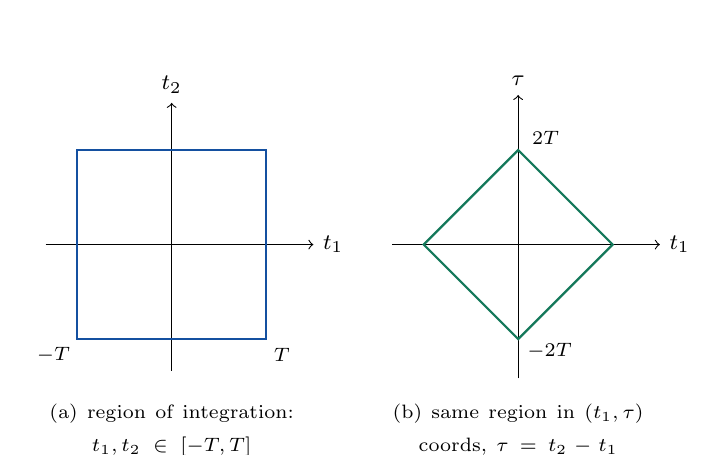
\begin{tikzpicture}
  % Panel (a): t1-t2 square
  \begin{scope}
    \draw[->] (-1.6,0) -- (1.8,0) node[right] {\footnotesize$t_1$};
    \draw[->] (0,-1.6) -- (0,1.8) node[above] {\footnotesize$t_2$};
    \draw[thick,defcol] (-1.2,-1.2) rectangle (1.2,1.2);
    \node at (1.4,-1.4) {\scriptsize $T$};
    \node at (-1.5,-1.4) {\scriptsize $-T$};
    \node[below, text width=3.4cm, align=center] at (0,-1.9) {\scriptsize (a) region of integration: $t_1,t_2\in[-T,T]$};
  \end{scope}
  \begin{scope}[xshift=4.4cm]
    \draw[->] (-1.6,0) -- (1.8,0) node[right] {\footnotesize$t_1$};
    \draw[->] (0,-1.7) -- (0,1.9) node[above] {\footnotesize$\tau$};
    \draw[thick,thmcol] (-1.2,0) -- (0,1.2) -- (1.2,0) -- (0,-1.2) -- cycle;
    \node at (0.35,1.35) {\scriptsize $2T$};
    \node at (0.4,-1.35) {\scriptsize $-2T$};
    \node[below, text width=3.6cm, align=center] at (0,-1.9) {\scriptsize (b) same region in $(t_1,\tau)$ coords, $\tau=t_2-t_1$};
  \end{scope}
\end{tikzpicture}
\end{center}

\begin{exbox}{Ergodicity worked examples (supplementary)}
\textbf{$X(t)=\cos(\omega t+\Theta)$, $\Theta\sim$Uniform$(0,2\pi)$:} mean $=0$ (constant),
$R_X(\tau)=\tfrac12\cos\omega\tau$ from \emph{both} the ensemble computation and the time-average
computation $\langle X(t)X(t+\tau)\rangle=\lim_{T\to\infty}\frac{1}{2T}\int_{-T}^{T}\cos(\omega
t+\theta)\cos(\omega t+\omega\tau+\theta)\,dt=\tfrac12\cos\omega\tau$ $\Rightarrow$
\textbf{ergodic}.\\[6pt]
\textbf{$R_{X}(\tau)=25+\dfrac{4}{1+6\tau^2}$ (stationary, ergodic, no periodic component):}
$\mu_X^2=\lim_{\tau\to\infty}R_X(\tau)=25\Rightarrow\mu_X=5$; $\E{X^2(t)}=R_X(0)=29
\Rightarrow \Var{X(t)}=29-25=4$.\\[6pt]
\textbf{$R_X(\tau)=A\delta(\tau)$, zero mean:} $\sigma_T^2=A/T\to0$ as $T\to\infty$
$\Rightarrow$ \textbf{mean-ergodic}.\\[6pt]
\textbf{Random binary transmission, $R(\tau)=1-|\tau|/T$:} $\Var{\bar X_T}=2/3\ne0$ even as
$T\to\infty$ $\Rightarrow$ \textbf{NOT mean-ergodic} (a triangular autocorrelation that never
decays relative to the averaging window fails the ergodic condition).
\end{exbox}

\keyresult{Exam pattern: you'll be given $R_X(\tau)$ and asked either (i) to find $\mu_X,
\Var{X(t)}$ using $\mu_X^2=\lim_{|\tau|\to\infty}R_X(\tau)$ and $R_X(0)=\E{X^2(t)}$, or (ii) to
decide ergodicity by checking whether $\Var{\bar X(T)}\to0$.}

\begin{exbox}{Valid autocorrelation functions? (quiz-style)}
Any candidate $R(\tau)$ \textbf{must} be even ($R(\tau)=R(-\tau)$) and satisfy
$|R(\tau)|\le R(0)$ (Theorem 13.12). A function like $R(\tau)=e^{-\tau^2}\sin\tau$ is
\textbf{odd} ($\sin$ is odd, $e^{-\tau^2}$ is even, product is odd) $\Rightarrow$
\textbf{not} a valid autocorrelation function --- purely even building blocks
($e^{-|\tau|}$, $e^{-\tau^2}$, $\cos\tau$, and products thereof) survive this test.
\end{exbox}

\clearpage
\section{Cross-Correlation (\S13.10)}
\label{sec:1310}

\begin{defbox}{13.17}{Cross-Correlation Function}
\[ R_{XY}(t,\tau) = \E{X(t)Y(t+\tau)}. \]
\end{defbox}

\begin{defbox}{13.18}{Jointly Wide Sense Stationary}
$X(t),Y(t)$ are jointly WSS if both are individually WSS \emph{and} $R_{XY}(t,\tau)=R_{XY}(\tau)$
depends only on $\tau$.
\end{defbox}

\begin{thmbox}{13.14}{Symmetry of Cross-Correlation}
If $X(t),Y(t)$ are jointly WSS: $\quad R_{XY}(\tau) = R_{YX}(-\tau)$.
\end{thmbox}

\begin{exbox}{13.24}{Noisy observation $Y(t)=X(t)+N(t)$: three WSS/jointly-WSS checks at once}
$X(t),N(t)$ independent WSS, $\mu_N=0$. Then $\E{Y(t)}=\mu_X$ (constant) and
\[
R_Y(t,\tau) = \E{[X(t)+N(t)][X(t+\tau)+N(t+\tau)]} = R_X(\tau)+R_N(\tau)
\]
(cross terms vanish by independence and $\mu_N=0$) $\Rightarrow$ \textbf{$Y(t)$ is WSS.}
Also $R_{YX}(t,\tau)=R_X(\tau)\Rightarrow$ \textbf{$X,Y$ jointly WSS}; and
$R_{YN}(t,\tau)=R_N(\tau)\Rightarrow$ \textbf{$Y,N$ jointly WSS}. \emph{(This is the standard
``signal plus independent noise'' template --- expect a variant of it on the exam.)}
\end{exbox}

\keyresult{Being individually WSS and being \emph{jointly} WSS with another process are two
separate checks --- always verify both from the definitions rather than assuming one implies
the other.}

\clearpage
\section{Gaussian Processes (\S13.11)}
\label{sec:1311}

\begin{defbox}{13.19}{Gaussian Process}
$X(t)$ is a Gaussian process iff $\mathbf{X}=[X(t_1)\ \cdots\ X(t_k)]'$ is a Gaussian random
vector for \emph{every} $k$ and every choice of $t_1,\dots,t_k$.
\end{defbox}

\begin{thmbox}{13.15}{A WSS Gaussian Process Is Stationary}
If $X(t)$ is a WSS Gaussian process, then $X(t)$ is (strict-sense) stationary.
\end{thmbox}
\begin{proof}
For any $t_1,\dots,t_k$ and shift $\tau$, WSS gives equal means and (since $C_X$ depends only
on the lag $t_j-t_i$) equal covariance matrices for $\mathbf X=[X(t_i)]$ and
$\tilde{\mathbf X}=[X(t_i+\tau)]$. A Gaussian vector's PDF is fully determined by its mean
vector and covariance matrix, so $f_{\mathbf X}=f_{\tilde{\mathbf X}}$ for arbitrary $k$ ---
i.e.\ stationary.
\end{proof}

\begin{defbox}{13.20}{White Gaussian Noise}
$W(t)$ is white Gaussian noise iff it is a stationary Gaussian process with $\mu_W=0$ and
$R_W(\tau)=\eta_0\delta(\tau)$. Consequence: samples at distinct times are \emph{independent}
Gaussians (uncorrelated $+$ jointly Gaussian $\Rightarrow$ independent, via Theorem 5.20).
Average power $R_W(0)=\eta_0\delta(0)=\infty$ --- physically impossible, but a useful
idealization.
\end{defbox}

\begin{flagbox}{Bivariate special case}{The Gaussian-process joint PDF reduces to Definition 5.10}
For a stationary Gaussian process, the joint PDF of any two samples $X_1=X(t)$, $X_2=X(t+\tau)$
is exactly the bivariate Gaussian PDF of \S\ref{sec:59} with $\sigma_1=\sigma_2=\sqrt{R_X(0)}$
and $\rho = C_X(\tau)/R_X(0)$. \textbf{Worked example:} $\mu_X(t)=0$, $R_X(\tau)=2^{-|\tau|}$.
Then $\Var{X(t)}=R_X(0)=1$, $\Cov{X(t),X(t+1)}=R_X(1)=1/2\Rightarrow\rho=1/2$, giving
\[ f_{X(t),X(t+1)}(x_1,x_2) = \frac{1}{\pi\sqrt3}\exp\!\left(-\frac{2(x_1^2-x_1x_2+x_2^2)}{3}\right). \]
\end{flagbox}

\subsection{Master Comparison Table: Which Processes Are Stationary / WSS?}

\begin{center}
\small
\begin{tabular}{@{}p{3.4cm}p{1.9cm}p{1.1cm}p{6.2cm}@{}}
\toprule
\textbf{Process} & \textbf{Station-ary?} & \textbf{WSS?} & \textbf{Why / why not}\\
\midrule
Random-phase carrier $A\cos(2\pi f_ct+\Theta)$, $\Theta\sim U(0,2\pi)$ & Not shown directly & \textbf{Yes} & $\mu_X=0$, $R_X(\tau)=\tfrac{A^2}{2}\cos2\pi f_c\tau$ (Ex.\ 13.22)\\[4pt]
White Gaussian noise & \textbf{Yes} & \textbf{Yes} & Gaussian $+$ WSS $\Rightarrow$ stationary (Thm 13.15)\\[4pt]
$W(t)=X(t)Y(t)$, $X,Y$ indep.\ WSS & Not shown directly & \textbf{Yes} & $R_W(\tau)=R_X(\tau)R_Y(\tau)$ (HW 13.10.1)\\[4pt]
$Y(t)=X(t-t_0)$, $X$ WSS & Not shown directly & \textbf{Yes} & $R_Y(\tau)=R_X(\tau)$: a delay doesn't change the ACF (HW 13.10.3)\\
\bottomrule
\end{tabular}
\end{center}

\clearpage
% ================================================================
\part{Full Exam \& Homework Problem Bank --- Every Problem, Fully Worked}
\label{part:exams}
% ================================================================

\begin{notebox}{How to Use This Part}
The professor said the final reuses the exact material from Exam 1 and Exam 2. Every problem
below is transcribed and solved completely, tagged with the theorem/section it exercises so
you can jump back to the relevant box above. The Chapter 13 homework set (\S13.9--13.11) is
included as well, since it directly exercises the professor-flagged WSS/cross-correlation/
Gaussian-process theorems.
\end{notebox}

\section{Exam 1 --- Full Solutions (7 Problems)}

\begin{examprob}{Exam 1, Problem 1}{Mixed random variable --- normalize, sketch CDF, compute probabilities \hfill [\S\ref{sec:delta}, Delta Functions/Mixed RVs]}
Given
\[ f_X(x) = \frac18\delta(x+2)+\frac{1}{16}\delta(x+1)+\frac1{16}\delta(x-1)+\begin{cases}Ax^2 & |x|\le2\\0&\text{otherwise}\end{cases}. \]

\textbf{(a) Find $A$.} Impulse probability totals $\frac18+\frac1{16}+\frac1{16}=\frac14$, so
the continuous part must supply $\frac34$:
\[ A\int_{-2}^{2}x^2\,dx = A\cdot\frac{16}{3} = \frac34 \ \Longrightarrow\ \boxed{A=\frac{9}{64}}. \]

\textbf{(b)/(c)/(d): full CDF} (built case-by-case, adding each impulse's jump as $x$ crosses it):
\[
F_X(x) = \begin{cases}
0 & x<-2\\[2pt]
\dfrac12+\dfrac{3x^3}{64} & -2\le x<-1\\[6pt]
\dfrac{9}{16}+\dfrac{3x^3}{64} & -1\le x<1\\[6pt]
\dfrac58+\dfrac{3x^3}{64} & 1\le x<2\\[2pt]
1 & x\ge2.
\end{cases}
\]
So $F_X(1)=\frac58+\frac{3}{64}=\boxed{\frac{43}{64}}$, and
$\P{-1<X\le2}=F_X(2)-F_X(-1)=1-\frac{33}{64}=\boxed{\frac{31}{64}}$.
\end{examprob}

\begin{examprob}{Exam 1, Problem 2}{Joint PDF, marginals, $\E{X},\E{X^2},\Var{X}$ \hfill [\S\ref{sec:57}--\ref{sec:58}]}
$f_{X,Y}(x,y)=\dfrac{x+y}{3}$ on $0\le x\le1,\ 0\le y\le2$.
\[ f_X(x) = \int_0^2\frac{x+y}{3}\,dy = \frac{2x+2}{3}, \qquad 0\le x\le1. \]
\[ \E{X} = \int_0^1 x\cdot\frac{2x+2}{3}\,dx=\frac59, \qquad
\E{X^2} = \int_0^1 x^2\cdot\frac{2x+2}{3}\,dx=\frac{7}{18}, \]
\[ \Var{X} = \frac{7}{18}-\left(\frac59\right)^2=\boxed{\frac{13}{162}}. \]
\end{examprob}

\begin{examprob}{Exam 1, Problem 3}{Joint PMF table --- marginals, $\E{Q}$, $\Var{G}$ \hfill [Joint/marginal PMF]}
Reconstructed joint PMF $P_{Q,G}(q,g)$: row sums $P_Q(0)=0.6,P_Q(1)=0.4$; column sums
$P_G(0){=}0.1,P_G(1){=}0.3,P_G(2){=}0.4,P_G(3){=}0.2$.
\[ \P{Q=0}=0.6,\quad \P{Q=G}=0.18,\quad \P{G=0}=0.1, \]
\[ \P{G>1}=0.6,\quad \P{G>Q}=0.78. \]
\[ \E{Q}=0.4. \qquad \E{G}=1.7,\ \E{G^2}=3.7\ \Longrightarrow\ \boxed{\Var{G}=3.7-1.7^2=0.81}. \]
\end{examprob}

\begin{examprob}{Exam 1, Problem 4}{Normalize a continuous PDF, CDF, probabilities \hfill [\S1, CDF/PDF basics]}
$f_X(x)=c(1-x^2)$ on $-1\le x\le1$. Normalizing: $c\int_{-1}^1(1-x^2)dx=\frac43c=1\Rightarrow
\boxed{c=\frac34}$.
\[ F_X(x)=\frac34\left[(x+1)-\frac13(x^3+1)\right]. \]
$\P{X=0}=0$ (continuous r.v.); $F_X(0)=\frac12$; $\P{0<X<0.5}=\frac{11}{32}$;
$\P{|X-\tfrac12|<\tfrac14}=\P{\tfrac14<X<\tfrac34}\approx0.2734$.
\end{examprob}

\begin{examprob}{Exam 1, Problem 5}{Bit-error probability: Gaussian noise, $Q$-function, SNR \hfill [\S\ref{sec:gaussian}]}
Bit-error probability $=Q(\sqrt{E/\sigma^2})$, SNR $=E/\sigma^2$.
\textbf{(a)} SNR$=4$: $Q(2)=1-\Phi(2)=1-0.97725=\boxed{0.02275}$.
\textbf{(b)} Need $Q(\sqrt{\text{SNR}})<10^{-6}\Rightarrow\sqrt{\text{SNR}}\ge4.75\Rightarrow
\boxed{\text{SNR}\ge(4.75)^2=22.56}$.
\end{examprob}

\begin{examprob}{Exam 1, Problem 6 (Extra Credit)}{Joint CDF --- solve for a normalizing constant \hfill [CDF properties]}
\[ F_{X,Y}(x,y)=a\left[\frac\pi2+\tan^{-1}\!\left(\frac x2\right)\right]\left[\frac\pi2+\tan^{-1}\!\left(\frac y3\right)\right]. \]
Using $\lim_{x,y\to\infty}F_{X,Y}(x,y)=1$ and $\tan^{-1}(\infty)=\pi/2$: $a\pi\cdot\pi=1
\Rightarrow \boxed{a=\dfrac{1}{\pi^2}}$. (Check: $F(-\infty,y)=F(x,-\infty)=0$ since
$\tan^{-1}(-\infty)=-\pi/2$.)
\end{examprob}

\begin{examprob}{Exam 1, Problem 7 (Extra Credit)}{Soft limiter --- Jacobian / inverse-function method \hfill [\S\ref{sec:63}]}
$Y=V(1-e^{-X/a})$ for $X\ge0$; $Y=-V(1-e^{X/a})$ for $X\le0$. Solving each branch for $x(y)$
and applying $f_Y(y)=f_X(x)\left|\dfrac{dx}{dy}\right|$:
\[
f_Y(y) = \frac{a}{V-y}\,f_X\!\left[a\ln\!\left(\frac{V}{V-y}\right)\right]u(y) \;+\;
\frac{a}{V+y}\,f_X\!\left[-a\ln\!\left(\frac{V}{V+y}\right)\right]u(-y).
\]
\end{examprob}

\clearpage
\section{Exam 2 --- Full Solutions (5 Problems)}

\begin{examprob}{Exam 2, Problem 1}{Joint PDF moments and covariance \hfill [\S\ref{sec:57}--\ref{sec:58}] --- textbook 5.7.12}
$f_{X,Y}(x,y)=4xy$ on the unit square.
\[ \E{X}=\E{Y}=\frac23, \qquad \E{X^2}=\E{Y^2}=\frac12 \ \Rightarrow\ \Var{X}=\Var{Y}=\frac1{18}. \]
\[ \E{XY}=\int_0^1\!\int_0^1 4x^2y^2\,dy\,dx = \frac49 \ \Rightarrow\ \Cov{X,Y}=\frac49-\left(\frac23\right)^2=0. \]
\[ \E{X+Y}=\frac43, \qquad \Var{X+Y}=\frac1{18}+\frac1{18}+2(0)=\boxed{\frac19}. \]
\end{examprob}

\begin{examprob}{Exam 2, Problem 2}{Bivariate-Gaussian-type joint PDF --- back out $\rho$, $\sigma$'s, $c$ \hfill [\S\ref{sec:59}] --- textbook 5.9.5}
$f_{X,Y}(x,y)=c\,e^{-(2x^2-4xy+4y^2)}$. Matching the exponent to Definition 5.10's quadratic
form: $\E{X}=\E{Y}=0$; solving the coefficient-matching equations gives
$\sigma_X=1/\sqrt2,\ \sigma_Y=1/2,\ \boxed{\rho=1/\sqrt2}$, and
\[ c = \frac{1}{2\pi\sigma_X\sigma_Y\sqrt{1-\rho^2}} = \boxed{\frac2\pi}. \]
Since $\rho\ne0$: \textbf{$X,Y$ are dependent} (by Theorem 5.20, since they're bivariate
Gaussian, uncorrelated would have been equivalent to independent --- but here they're
correlated).
\end{examprob}

\begin{examprob}{Exam 2, Problem 3}{Power dissipation $Y=9X^2$, then range-limited $W$ \hfill [\S\ref{sec:62}--\ref{sec:63}] --- textbook 6.3.10}
$X\sim$Uniform$(-2,2)$ (current), $Y=9X^2$ (power, Watts). Following the Example 6.4 template
exactly (with $c=9$): $0\le Y<36$, and for $0\le y<36$,
\[ F_Y(y)=\P{-\tfrac{\sqrt y}{3}\le X\le\tfrac{\sqrt y}{3}} = \frac{\sqrt y}{6}
\ \Longrightarrow\ f_Y(y)=\frac{1}{12\sqrt y},\quad 0<y\le36. \]
\textbf{Range-limited} $W=Y$ if $Y<16$, else $W=16$: for $0\le w<16$, $F_W(w)=F_Y(w)=\sqrt
w/6$; at $w=16$ there's a jump from $F_W(16^-)=4/6$ to $1$, i.e.\ an impulse of weight
$1-\frac46=\frac13$:
\[ f_W(w) = \frac{1}{12\sqrt w}\ (0\le w<16) \;+\; \frac13\delta(w-16). \]
\emph{(This is the exact soft-limiter/impulse-weight technique of Example 6.8, applied on top
of the $Y{=}cX^2$ technique of Example 6.4.)}
\end{examprob}

\begin{examprob}{Exam 2, Problem 4}{Joint PDF on a triangle --- correlation and $\E{e^{X+Y}}$ \hfill [\S\ref{sec:58}] --- textbook 5.8.8}
$f_{X,Y}(x,y)=\frac12$ on $-1\le x\le y\le1$.
\[ r_{X,Y}=\E{XY} = \frac14\int_{-1}^1 x(1-x^2)\,dx = \boxed{0} \qquad(\text{odd integrand}). \]
\[ \E{e^{X+Y}} = \frac12\int_{-1}^{1} e^x(e-e^x)\,dx = \boxed{\frac{e^2}{4}+\frac{e^{-2}}{4}-\frac12}. \]
\end{examprob}

\begin{examprob}{Exam 2, Problem 5}{Discrete joint PMF --- full moment/covariance workup \hfill [\S\ref{sec:58}] --- textbook 5.8.6}
$P_{X,Y}(x,y)=1/(4x)$ for integers $1\le y\le x\le4$.
\[ \E{X}=\frac52,\ \E{Y}=\frac74, \qquad \Var{X}=\frac54,\ \Var{Y}=\frac{41}{48}. \]
\[ r_{X,Y}=\E{XY}=5 \ \Longrightarrow\ \Cov{X,Y}=5-\left(\frac74\right)\!\left(\frac{10}4\right)=\frac{10}{16}. \]
\[ \rho_{X,Y} = \frac{10/16}{\sqrt{(5/4)(41/48)}} \approx \boxed{0.605}. \]
\end{examprob}

\clearpage
\section{Chapter 13 Homework --- Full Solutions (6 Problems)}

\begin{examprob}{Problem 13.9.1}{Which of the following are valid autocorrelation functions? \hfill [\S\ref{sec:139}, Theorem 13.12]}
$R_1(\tau)=\delta(\tau)$, $\ R_2(\tau)=\delta(\tau)+10$, $\ R_3(\tau)=\delta(\tau-10)$, $\
R_4(\tau)=\delta(\tau)-10$.

Test every candidate against Theorem 13.12: must be even ($R(\tau)=R(-\tau)$), and (from the
supplementary ergodic-process properties) if $X(t)$ has nonzero mean and no periodic
component, $\lim_{|\tau|\to\infty}R_X(\tau)=\mu_X^2\ge0$.

\textbf{$R_1(\tau)=\delta(\tau)$:} even ($\delta(\tau)=\delta(-\tau)$) --- this is exactly the
white-noise autocorrelation of Definition 13.20 (with $\eta_0=1$). \textbf{Valid.}

\textbf{$R_2(\tau)=\delta(\tau)+10$:} even. It is the sum of two individually valid
autocorrelations --- $\delta(\tau)$ (white noise) and the constant $10$ (the autocorrelation
of a ``process'' that is a random constant $A$ with $\E{A^2}=10$, so $R_A(\tau)=\E{A\cdot
A}=10$ for all $\tau$). The autocorrelation of a sum of two \emph{independent} processes is
the sum of their autocorrelations, so $R_2$ is realizable. \textbf{Valid.}

\textbf{$R_3(\tau)=\delta(\tau-10)$:} $R_3(-\tau)=\delta(-\tau-10)=\delta(\tau+10)\ne
\delta(\tau-10)=R_3(\tau)$ --- \textbf{fails the evenness property outright.} \textbf{Not
valid.}

\textbf{$R_4(\tau)=\delta(\tau)-10$:} even ($\delta(\tau)-10=\delta(-\tau)-10$), so it passes
that test. But away from the origin ($\tau\ne0$) $R_4(\tau)=-10$ for \emph{every} nonzero lag,
so $\lim_{|\tau|\to\infty}R_4(\tau)=-10$. Since this limit must equal $\mu_X^2\ge0$ for any
real process, $-10<0$ is impossible. \textbf{Not valid.}

\boxed{\text{Valid: } R_1, R_2. \qquad \text{Not valid: } R_3, R_4.}
\end{examprob}

\begin{examprob}{Problem 13.9.5}{iid sequence $X_n$: find $R_X[n,k]$ \hfill [Definition 13.13, Theorem 4.5(c)]}
$X_n$ is iid with $\E{X_n}=\mu$, $\Var{X_n}=\sigma^2$. Find $R_X[n,k]=\E{X_nX_{n+k}}$.

\textbf{Case $k=0$:} $R_X[n,0]=\E{X_n^2}=\Var{X_n}+(\E{X_n})^2=\sigma^2+\mu^2$ (Theorem
4.5(c)).

\textbf{Case $k\ne0$:} $X_n$ and $X_{n+k}$ are \emph{independent} (different terms of an iid
sequence), so by Theorem 5.17(b), $R_X[n,k]=\E{X_n}\E{X_{n+k}}=\mu^2$.

\[
\boxed{R_X[n,k] = \begin{cases}\sigma^2+\mu^2 & k=0\\ \mu^2 & k\ne0.\end{cases}}
\]
Independent of $n$: this confirms an iid sequence is (trivially) stationary, since every
finite joint PDF is a product of identical marginals, hence shift-invariant.
\end{examprob}

\begin{examprob}{Problem 13.9.9}{WSS process modulated by an independent random phase \hfill [Example 13.22's lemma, Theorem 13.16]}
$X(t)$ is WSS with average power $R_X(0)=\E{X^2(t)}=1$. $\Theta\sim$Uniform$(0,2\pi)$,
independent of $X(t)$.

\textbf{(a)} $\E{X^2(t)}=R_X(0)=\boxed{1}$ (given directly --- this is Definition 13.16's
average power).

\textbf{(b)} Using Example 13.22's lemma with $a=2\pi f_ct$, $k=1$:
\[ \E{\cos(2\pi f_ct+\Theta)} = \int_0^{2\pi}\cos(2\pi f_ct+\theta)\frac{d\theta}{2\pi} = \boxed{0}. \]

\textbf{(c)} $Y(t)=X(t)\cos(2\pi f_ct+\Theta)$. Since $X(t)$ and $\Theta$ are independent,
Theorem 5.17(a) gives
\[ \E{Y(t)} = \E{X(t)}\cdot\E{\cos(2\pi f_ct+\Theta)} = \E{X(t)}\cdot 0 = \boxed{0} \]
regardless of $\E{X(t)}$.

\textbf{(d)} Average power of $Y(t)$: $\E{Y^2(t)}=\E{X^2(t)\cos^2(2\pi f_ct+\Theta)}$.
Independence again gives $\E{Y^2(t)}=\E{X^2(t)}\cdot\E{\cos^2(2\pi f_ct+\Theta)}$. Using
$\cos^2\phi=\tfrac12[1+\cos2\phi]$ and the lemma with $a=4\pi f_ct$, $k=2$:
\[ \E{\cos^2(2\pi f_ct+\Theta)} = \frac12+\frac12\E{\cos(4\pi f_ct+2\Theta)} = \frac12+0 = \frac12. \]
So average power $=\E{X^2(t)}\cdot\tfrac12 = 1\cdot\tfrac12 = \boxed{1/2}$.
\end{examprob}

\begin{examprob}{Problem 13.10.1}{Product of two independent WSS processes \hfill [Definitions 13.11--13.13, 13.17--13.18]}
$X(t),Y(t)$ independent WSS with means $\mu_X,\mu_Y$ and autocorrelations $R_X(\tau),R_Y(\tau)$.
$W(t)=X(t)Y(t)$.

\textbf{(a)} By independence (Theorem 5.17(a)):
\[ \mu_W = \E{W(t)} = \E{X(t)}\E{Y(t)} = \mu_X\mu_Y \quad\text{(constant).} \]
\[
R_W(t,\tau) = \E{W(t)W(t+\tau)} = \E{X(t)Y(t)X(t+\tau)Y(t+\tau)}
\]
\[
= \E{X(t)X(t+\tau)}\cdot\E{Y(t)Y(t+\tau)} = R_X(\tau)R_Y(\tau),
\]
using independence of the $X$ and $Y$ processes to split the expectation of the product.
$R_W(t,\tau)=R_X(\tau)R_Y(\tau)$ depends only on $\tau$, and $\mu_W$ is constant, so
\boxed{W(t)\text{ is WSS.}}

\textbf{(b)} Cross-correlation of $W$ and $X$:
\[
R_{WX}(t,\tau) = \E{W(t)X(t+\tau)} = \E{X(t)Y(t)X(t+\tau)} = \E{X(t)X(t+\tau)}\cdot\E{Y(t)}
= R_X(\tau)\mu_Y,
\]
using independence of $Y(t)$ from $X(t),X(t+\tau)$. This depends only on $\tau$, and both
$W(t)$ and $X(t)$ are individually WSS, so \boxed{\text{yes, jointly WSS.}}
\end{examprob}

\begin{examprob}{Problem 13.10.3}{Autocorrelation/cross-correlation of a time-delayed WSS process \hfill [Definitions 13.13, 13.17--13.18]}
$X(t)$ WSS with $R_X(\tau)=10\sin(2\pi\cdot1000\tau)/(2\pi\cdot1000\tau)$. $Y(t)=X(t-t_0)$,
$t_0=5\times10^{-5}$s.

\textbf{(a)} $R_Y(t,\tau)=\E{Y(t)Y(t+\tau)}=\E{X(t-t_0)X(t+\tau-t_0)}$. The two arguments of
$X$ differ by exactly $\tau$ (independent of $t_0$), and $X$ is WSS, so
\[ \boxed{R_Y(\tau) = R_X(\tau) = \frac{10\sin(2\pi\cdot1000\tau)}{2\pi\cdot1000\tau}.} \]
\emph{Delaying a WSS process does not change its autocorrelation function.}

\textbf{(b)} $R_{XY}(t,\tau)=\E{X(t)Y(t+\tau)}=\E{X(t)X(t+\tau-t_0)}$. The two arguments of
$X$ now differ by $\tau-t_0$, so
\[ \boxed{R_{XY}(\tau) = R_X(\tau-t_0) = \frac{10\sin\!\big(2\pi\cdot1000(\tau-t_0)\big)}{2\pi\cdot1000(\tau-t_0)}.} \]

\textbf{(c)} From (a), $R_Y(\tau)$ depends only on $\tau$, and $\mu_Y=\E{X(t-t_0)}=\mu_X$
(constant, since $X$ is WSS). \boxed{\text{Yes, } Y(t)\text{ is WSS.}}

\textbf{(d)} From (b), $R_{XY}(t,\tau)=R_X(\tau-t_0)$ depends only on $\tau$ (not on $t$), and
both $X(t),Y(t)$ are individually WSS. \boxed{\text{Yes, jointly WSS.}}
\end{examprob}

\begin{examprob}{Problem 13.11.2}{Which transformations of a Gaussian process stay Gaussian? \hfill [Definition 13.19, Theorem 5.21/8.11]}
Given a Gaussian process $X(t)$, identify which are Gaussian processes: (a) $2X(t)$,
(b) $X(t/2)$, (c) $X(t)/2$, (d) $X(t)-X(t-1)$, (e) $X(2t)$.

By Definition 13.19, a process $Z(t)$ is Gaussian iff $[Z(t_1),\dots,Z(t_k)]'$ is a Gaussian
random vector for \emph{every} choice of $k$ time instants. Two facts do all the work:
(i) \textbf{re-indexing time} (evaluating $X$ at a different, still-arbitrary set of time
instants) trivially preserves the ``any finite sample vector is Gaussian'' property; (ii) a
\textbf{linear transformation} of a Gaussian vector is again a Gaussian vector
(Theorem 5.21/8.11).

\textbf{(a) $2X(t)$:} for any $t_1,\dots,t_k$, $[2X(t_1),\dots,2X(t_k)]'$ is a linear
(scalar) transform of the Gaussian vector $[X(t_1),\dots,X(t_k)]'$. \boxed{\text{Gaussian.}}

\textbf{(b) $X(t/2)$:} for any $t_1,\dots,t_k$, $[X(t_1/2),\dots,X(t_k/2)]'$ is simply a
sample of $X$ at the (still arbitrary) time instants $t_1/2,\dots,t_k/2$ --- Gaussian by
Definition 13.19 directly. \boxed{\text{Gaussian.}}

\textbf{(c) $X(t)/2$:} same as (a) with scalar $1/2$. \boxed{\text{Gaussian.}}

\textbf{(d) $X(t)-X(t-1)$:} for any $t_1,\dots,t_k$, $[X(t_1)-X(t_1-1),\dots,
X(t_k)-X(t_k-1)]'$ is a linear transformation of the $2k$-dimensional Gaussian vector
$[X(t_1),X(t_1-1),\dots,X(t_k),X(t_k-1)]'$ (itself Gaussian, being $2k$ samples of $X$).
\boxed{\text{Gaussian.}}

\textbf{(e) $X(2t)$:} same reasoning as (b), sampling $X$ at times $2t_1,\dots,2t_k$.
\boxed{\text{Gaussian.}}

\textbf{All five are Gaussian processes.} \emph{Lesson: the Gaussian-process property is
extremely robust --- it survives any linear operation on the values and any re-indexing
(including nonlinear re-indexing like $t\mapsto2t$) of the time axis.}
\end{examprob}

\clearpage
% ================================================================
\part{Formula Cheat Sheet}
\label{part:cheatsheet}
% ================================================================
\section*{Master Formula Reference (all chapters, one place)}
\addcontentsline{toc}{section}{Master Formula Reference}

\small
\begin{longtable}{@{}p{4.0cm}p{10.2cm}@{}}
\toprule
\textbf{Topic} & \textbf{Formula} \\
\midrule
\endhead
CDF & $F_X(x)=\P{X\le x}$; $\P{x_1{<}X{\le}x_2}=F_X(x_2)-F_X(x_1)$\\
PDF & $f_X(x)=dF_X/dx$; $\int f_X=1$; $F_X(x)=\int_{-\infty}^x f_X$\\
Expectation & $\E{X}=\int xf_X(x)dx$; $\E{g(X)}=\int g(x)f_X(x)dx$\\
Variance & $\Var{X}=\E{X^2}-(\E{X})^2$; $\Var{aX+b}=a^2\Var{X}$\\
Gaussian PDF & $f_X(x)=\dfrac{1}{\sqrt{2\pi}\sigma}e^{-(x-\mu)^2/2\sigma^2}$; $F_X(x)=\Phi\!\left(\frac{x-\mu}{\sigma}\right)$\\
$Q$-function & $Q(z)=1-\Phi(z)=\P{Z>z}$; $\Phi(-z)=1-\Phi(z)$\\
Delta/sifting & $\int g(x)\delta(x-x_0)dx=g(x_0)$; discrete PDF $=\sum P_X(x_i)\delta(x-x_i)$\\
Mixed RV & PDF has impulses \emph{and} nonzero finite values\\
$\E{g(X,Y)}$ & $\iint g(x,y)f_{X,Y}(x,y)\,dx\,dy$\\
$\E{X+Y}$ & $=\E{X}+\E{Y}$ always (even if dependent)\\
$\Var{X+Y}$ & $=\Var{X}+\Var{Y}+2\Cov{X,Y}$ --- needs the joint model\\
Covariance & $\Cov{X,Y}=\E{XY}-\E{X}\E{Y}$\\
Correlation & $r_{X,Y}=\E{XY}$\\
Correlation coeff. & $\rho_{X,Y}=\Cov{X,Y}/(\sigma_X\sigma_Y)\in[-1,1]$\\
Independent $\Rightarrow$ & $\Cov{X,Y}=\rho_{X,Y}=0$ (uncorrelated) --- converse false in general\\
Bivariate Gaussian & $f_{X,Y}(x,y)=\dfrac{\exp\!\left[-Q(x,y)/2(1-\rho^2)\right]}{2\pi\sigma_X\sigma_Y\sqrt{1-\rho^2}}$, \ where $Q(x,y)=\left(\frac{x-\mu_X}{\sigma_X}\right)^2-\frac{2\rho(x-\mu_X)(y-\mu_Y)}{\sigma_X\sigma_Y}+\left(\frac{y-\mu_Y}{\sigma_Y}\right)^2$ (full form: see \S\ref{sec:59})\\
Bivar.\ Gaussian, unc.\ $\Leftrightarrow$ ind. & only family where this equivalence holds\\
$F_W(w)$, $W=g(X)$ & $F_W(w)=\P{g(X)\le w}$, then differentiate\\
$W=aX+b$ & $f_W(w)=\frac1{|a|}f_X\!\left(\frac{w-b}a\right)$\\
$W=X^2$ (or $cX^2$) & $F_W(w)=\P{-\sqrt{w/c}\le X\le\sqrt{w/c}}$, clip to $X$'s support, differentiate piecewise\\
Range-limited/clipped $W$ & continuous part unchanged where active; impulse of weight $=$ clipped tail probability at each clip point\\
Mean function & $\mu_X(t)=\E{X(t)}$\\
Autocorrelation & $R_X(t,\tau)=\E{X(t)X(t+\tau)}$; $R_X(t,0)=\E{X^2(t)}$ (power)\\
Autocovariance & $C_X(t,\tau)=R_X(t,\tau)-\mu_X(t)\mu_X(t+\tau)$\\
Stationary & every joint PDF is shift-invariant in $t$\\
WSS & $\mu_X(t)=\mu_X$ (const.) and $R_X(t,\tau)=R_X(\tau)$\\
WSS autocorrelation & $R_X(0)\ge0$; $R_X(\tau)=R_X(-\tau)$; $R_X(0)\ge|R_X(\tau)|$\\
Ergodic (mean) & $\lim_{T\to\infty}\bar X(T)=\mu_X=\E{X(t)}$ and similarly for $\E{X^2(t)}$\\
Cross-correlation & $R_{XY}(t,\tau)=\E{X(t)Y(t+\tau)}$; jointly WSS $\Rightarrow R_{XY}(\tau)=R_{YX}(-\tau)$\\
Gaussian process & every finite sample vector $[X(t_1)\cdots X(t_k)]'$ is Gaussian; WSS $+$ Gaussian $\Rightarrow$ stationary\\
\bottomrule
\end{longtable}
\normalsize

\vspace{10pt}
\begin{center}
\fcolorbox{flagcol}{flagbg}{\parbox{0.9\linewidth}{\centering
\textbf{\color{flagcol}The Professor's Three Flagged Chapter-13 Theorems, One More Time}\\[6pt]
\textbf{Thm 13.10:} stationary $X(t)\Rightarrow aX(t)+b$ stationary $(a>0)$.\qquad
\textbf{Thm 13.11:} stationary $\Rightarrow$ const.\ mean $+$ $R_X(t,\tau){=}R_X(\tau)$.\qquad
\textbf{Thm 13.12:} WSS $\Rightarrow$ $R_X(0){\ge}0$, even, peak at $0$.\qquad
\textbf{Ex.\ 13.22:} $A\cos(2\pi f_ct+\Theta)$, $\Theta\sim U(0,2\pi)$, is WSS with
$R_X(\tau)=\tfrac{A^2}2\cos2\pi f_c\tau$.
}}
\end{center}

\clearpage
\section*{10 Rapid Self-Check Questions (Chapter 13, with answers)}
\addcontentsline{toc}{section}{Rapid Self-Check Questions}
\begin{enumerate}
\item[1.] A process where both $X$ and $t$ are continuous is a \emph{continuous random
process}.
\item[2.] A process whose future is fully determined by its past sample values is
\emph{deterministic}.
\item[3.] A process whose statistical properties don't change with time is
\emph{stationary}.
\item[4.] A first-order stationary process has a \emph{constant mean}.
\item[5.] $R_{XX}(t_1,t_2)=\E{X(t_1)X(t_2)}$.
\item[6.] Ensemble averages equal time averages $\Rightarrow$ \emph{(mean-)ergodic}.
\item[7.] For WSS processes, $R_{XX}(0)=\E{X^2(t)}$.
\item[8.] $|R_{XY}(\tau)|\le\sqrt{R_{XX}(0)R_{YY}(0)}$ \textbf{and}
$|R_{XY}(\tau)|\le\tfrac12[R_{XX}(0)+R_{YY}(0)]$ --- both true (the first is tighter, since
geometric mean $\le$ arithmetic mean).
\item[9.] A WSS noise process with constant power density spectrum is \emph{white noise}.
\item[10.] Band-limited sampling frequency $\omega_s = 2\pi/T_s$.
\end{enumerate}

\clearpage
\section*{Final Reminders}
\addcontentsline{toc}{section}{Final Reminders}
\begin{itemize}
\item The professor's choice section draws from \textbf{Ch.\ 4, 5, 6} --- know CDF/PDF basics,
Gaussian RVs, delta/mixed RVs (Ch.\ 4); joint expectation, covariance/correlation, bivariate
Gaussian (Ch.\ 5); and the $F_W\to f_W$ derivation method including power/limiter problems
(Ch.\ 6) cold.
\item \textbf{Two guaranteed questions on Chapter 13} --- prioritize Theorems 13.10, 13.11,
13.12, Example 13.22, the WSS definition, and the ergodicity concept above everything else in
that chapter.
\item Always ask three questions on a Ch.\ 13 problem: (1) Is the mean constant? (2) Does
$R_X$ depend on $t$, or only on $\tau=$ the time difference? (3) If both yes, it's WSS ---
then check evenness/peak-at-zero (Thm 13.12) or ergodicity as asked.
\item On Ch.\ 6 problems, always start with the two-step method: find $F_W(w)=\P{g(X)\le w}$,
then differentiate --- and watch for clipped/range-limited variables, which add an impulse at
the clip point.
\end{itemize}

\end{document}
